% This is text associated with the open textbook "Open Electromagnetics"
% See immediately below for author, date
% This work is licensed under the Creative Commons Attribution-ShareAlike 4.0 International License. (CC BY-SA 4.0) 
% To view a copy of the license, visit http://creativecommons.org/licenses/by-sa/4.0/

%ORB TITLE Standing Waves
%ORB AUTHOR 0        # S.W. Ellingson, Virginia Tech (ellingson@vt.edu)
%ORB DATE 20180802   # yyyymmdd
%ORB ABSTRACT Standing waves concept, examples 

\label{m0086_Standing_Waves}  % <-- Must match name of this file and module directory name.  Don't mess with this!
\index{standing wave|(}

%ORB HIGHLIGHT
\begin{mdframed}[backgroundcolor=yellow!20,nobreak=true] 
A \emph{standing wave} 
\index{standing wave!definition}
consists of waves moving in opposite directions.  These waves add to make a distinct magnitude variation as a function of distance that does not vary in time. 
\end{mdframed}

To see how this can happen, first consider that an incident wave $V_0^+ e^{-j\beta z}$, which is traveling in the $+z$ axis along a lossless transmission line.
Associated with this wave is a reflected wave $V_0^- e^{+j\beta z}=\Gamma V_0^+ e^{+j\beta z}$, where $\Gamma$ is the voltage reflection coefficient. 
These waves add to make the total potential
%
\begin{equation}
\begin{split}
\widetilde{V}(z) & = V_0^+ e^{-j\beta z} + \Gamma V_0^+ e^{+j\beta z} \\
                 & = V_0^+ \left( e^{-j\beta z} + \Gamma e^{+j\beta z} \right) 
\end{split}
\end{equation}
%
The magnitude of $\widetilde{V}(z)$ is most easily found by first finding $|\widetilde{V}(z)|^2$, which is:
%
\begin{flalign}
  &\widetilde{V}(z) \widetilde{V}^*(z) \nonumber \\
= &|V_0^+|^2 \left( e^{-j\beta z} + \Gamma e^{+j\beta z} \right)  \left( e^{-j\beta z} + \Gamma e^{+j\beta z} \right)^* \nonumber \\
= &|V_0^+|^2 \left( e^{-j\beta z} + \Gamma e^{+j\beta z} \right)  \left( e^{+j\beta z} + \Gamma^* e^{-j\beta z} \right) \nonumber \\
= &|V_0^+|^2 \left( 1 + \left|\Gamma\right|^2 + \Gamma e^{+j2\beta z} + \Gamma^* e^{-j2\beta z}  \right) 
\end{flalign}
%
Let $\phi$ be the phase of $\Gamma$; i.e., 
%
\begin{equation}
\Gamma = \left|\Gamma\right|e^{j\phi}
\end{equation}
%
Then, continuing from the previous expression:
%
\begin{flalign}
  &|V_0^+|^2 \left( 1 + \left|\Gamma\right|^2 + \left|\Gamma\right| e^{+j\left(2\beta z+\phi\right)} + \left|\Gamma\right| e^{-j\left(2\beta z+\phi\right)}  \right) \nonumber \\
= &|V_0^+|^2 \left( 1 + \left|\Gamma\right|^2 + \left|\Gamma\right| \left[ e^{+j\left(2\beta z+\phi\right)} + e^{-j\left(2\beta z+\phi\right)} \right]  \right) 
\end{flalign}
%
The quantity in square brackets can be reduced to a cosine function using the identity 
%
\begin{equation}
\cos\theta = \frac{1}{2}\left[e^{j\theta}+e^{-j\theta}\right]
\nonumber
\end{equation}
%
yielding:
%
\begin{equation}
|V_0^+|^2 \left[ 1 + \left|\Gamma\right|^2 + 2\left|\Gamma\right| \cos\left( 2\beta z + \phi \right) \right] 
\end{equation}
% 
Recall that this is $|\widetilde{V}(z)|^2$. $|\widetilde{V}(z)|$ is therefore the square root of the above expression:
%
\begin{equation}
\left|\widetilde{V}(z)\right| = |V_0^+| \sqrt{ 1 + \left|\Gamma\right|^2 + 2\left|\Gamma\right| \cos\left( 2\beta z + \phi \right) } 
\end{equation}
%
Thus, we have found that the magnitude of the resulting total potential varies sinusoidally along the line.  
This is referred to as a standing wave because the variation of the magnitude of the phasor resulting from the interference between the incident and reflected waves does not vary with time.

We may perform a similar analysis of the current, leading to:
%
\begin{equation}
\left|\widetilde{I}(z)\right| = \frac{|V_0^+|}{Z_0} \sqrt{ 1 + \left|\Gamma\right|^2 - 2\left|\Gamma\right| \cos\left( 2\beta z + \phi \right) } 
\end{equation}
%
%TODO Problem: {\color{red}(PROBLEM: student do this)}
Again we find the result is a standing wave.

Now let us consider the outcome for a few special cases.  

{\bf Matched load.} When the impedance of the termination of the transmission line, $Z_L$, is equal to the characteristic impedance of the transmission line, $Z_0$, $\Gamma=0$ and there is no reflection. In this case, the above expressions reduce to $|\widetilde{V}(z)| = |V_0^+|$ and $|\widetilde{I}(z)| = |V_0^+|/Z_0$, as expected.

{\bf Open or Short-Circuit.}
\index{open circuit}
\index{short circuit}
In this case, $\Gamma=\pm1$ and we find:
%
\begin{equation}
\left|\widetilde{V}(z)\right| = |V_0^+| \sqrt{ 2 + 2\cos\left( 2\beta z + \phi \right) } 
\end{equation} 
%
\begin{equation}
\left|\widetilde{I}(z)\right| = \frac{|V_0^+|}{Z_0} \sqrt{ 2 - 2\cos\left( 2\beta z + \phi \right) } 
\end{equation}  
%
where $\phi=0$ for an open circuit and $\phi=\pi$ for a short circuit.  
The result for an open circuit termination is shown in Figure~\ref{m0086_fStandingWaveOC}(a) (potential) and \ref{m0086_fStandingWaveOC}(b) (current).
The result for a short circuit termination is identical except the roles of potential and current are reversed.
In either case, note that voltage maxima correspond to current minima, and vice versa.
%
\begin{figure}
\begin{center}
%\pdftooltip{{  % note double braces
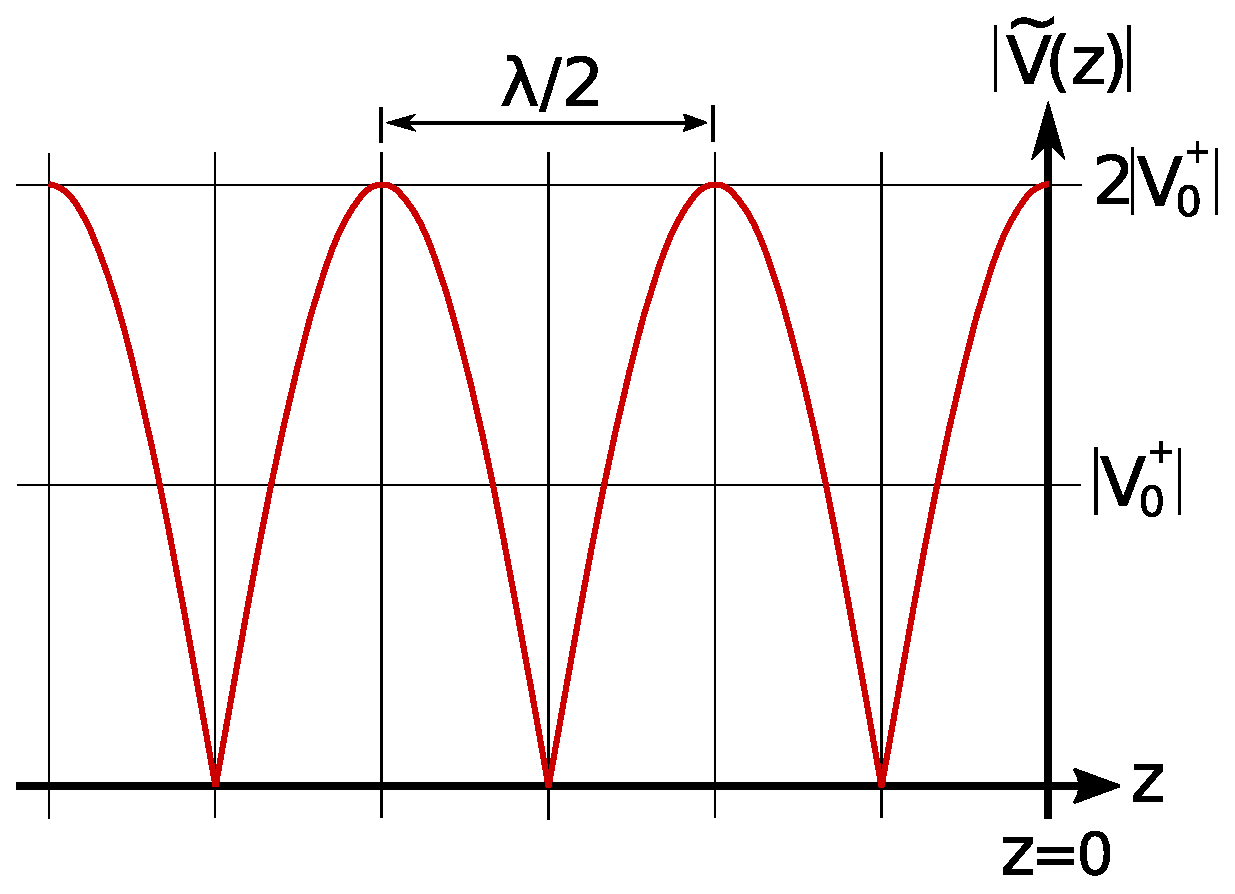
\includegraphics[width=2.5in]{modules/m0086_fStandingWaveOC-V.eps}\\
%}}{The figure shows two plots, one above the other (a and b). Graph (a) shows the potential, with z=0 as the x-axis and the absolute value of the alternating voltage on the y-axis. 
%%The graph depicts a half standing wave, followed by two full standing waves and another half wave. 
%The top peak of the wave reaches twice the absolute value of V super + sub 0, with the absolute value of V super + sub 0 at the midpoint. 
%%Wavelength (lambda) is measured from the peak of the two full peaks. 
%Graph (b) shows the current, and features z=0 on the x-axis and the absolute value of the alternating current on the y-axis. 
%The graph depicts %three full standing waves, with the 
%peaks at twice the absolute value of I super + sub 0. 
%%Wavelength (lambda) is measured from the left minimum of the middle wave to the right minimum of the middle wave. 
%}
(a) Potential.\\~\\
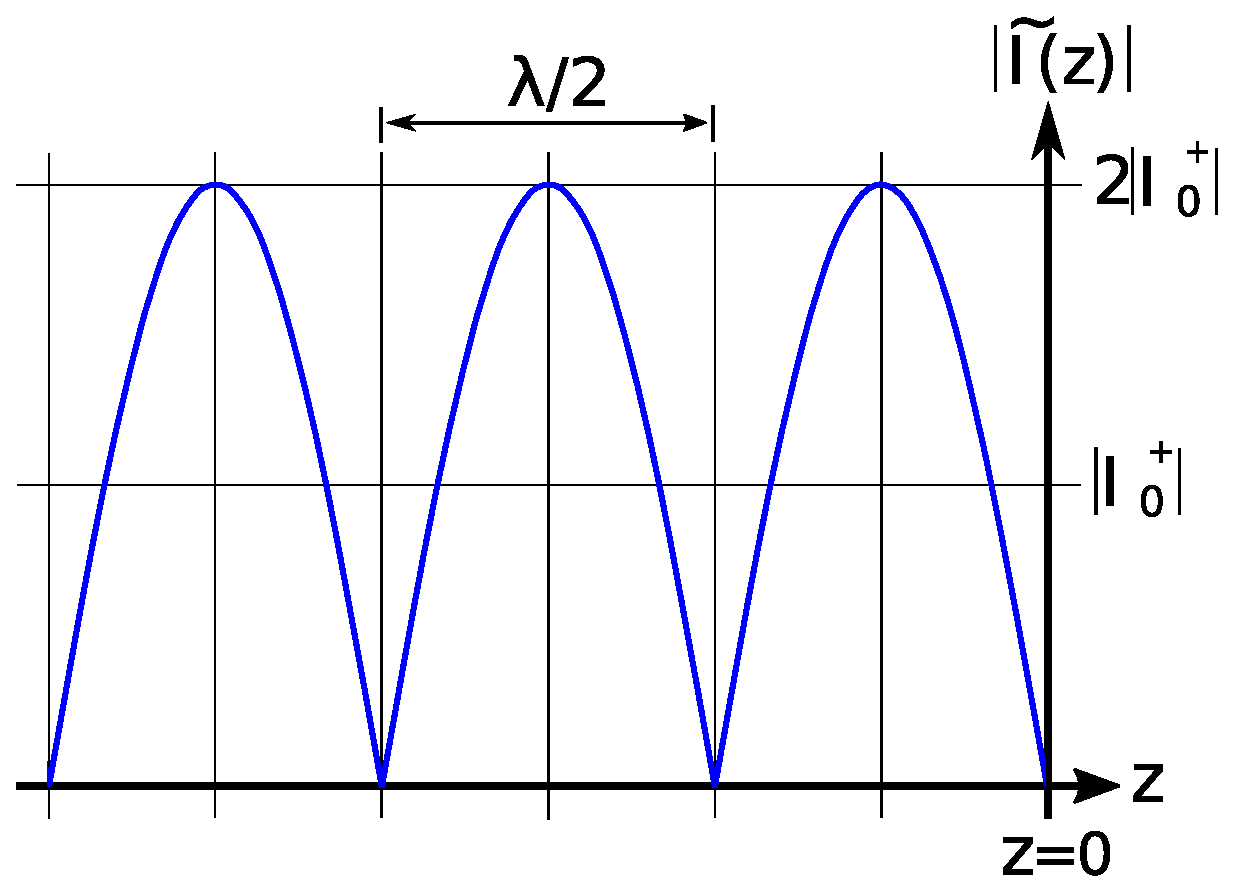
\includegraphics[width=2.5in]{modules/m0086_fStandingWaveOC-C.eps}\\
(b) Current.
\end{center} 
\caption{\label{m0086_fStandingWaveOC}Standing wave associated with an open-circuit termination at $z=0$ (incident wave arrives from left).}
\end{figure} 

Also note: 
%
%ORB HIGHLIGHT
\begin{mdframed}[backgroundcolor=yellow!20,nobreak=true] 
The period of the standing wave is $\lambda/2$; i.e., one-half of a wavelength.
\end{mdframed}
%
This can be confirmed as follows.
First, note that the frequency argument of the cosine function of the standing wave is $2\beta z$.
This can be rewritten as $2\pi\left(\beta/\pi\right)z$, so the frequency of variation is $\beta/\pi$ and the period of the variation is $\pi/\beta$.
Since $\beta=2\pi/\lambda$, we see that the period of the variation is $\lambda/2$.
Furthermore, this is true regardless of the value of $\Gamma$.

{\bf Mismatched loads.} A common situation is that the termination is neither perfectly-matched ($\Gamma=0$) nor an open/short circuit ($\left|\Gamma\right|=1$).
Examples of the resulting standing waves are shown in Figure~\ref{m0086_fStandingWaveExample}. 
%
\begin{figure}
\begin{center}
\pdftooltip{{  % note double braces
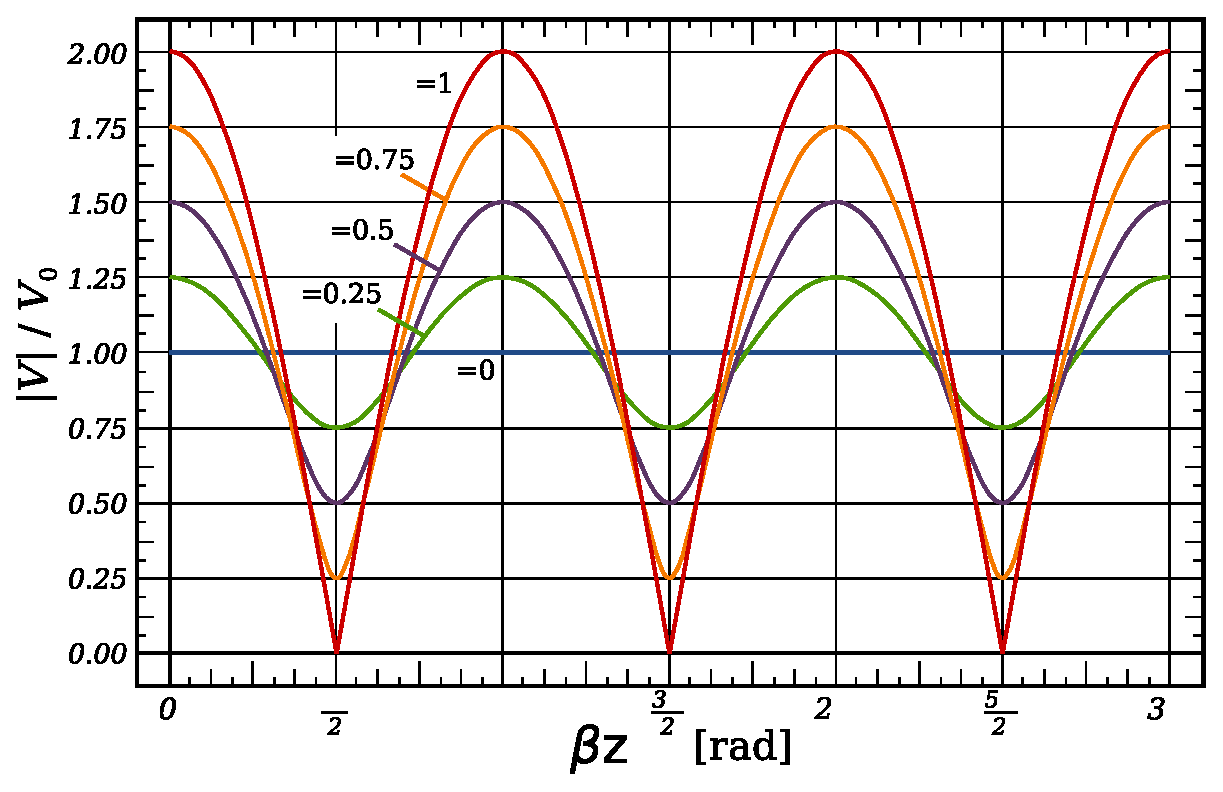
\includegraphics[width=\columnwidth]{modules/m0086_fStandingWaves.eps}
% https://commons.wikimedia.org/wiki/File:Standing_Wave_Ratio.svg
}}{Standing waves plotted: the x-axis (beta sub z) goes from 0 to 3*pi in one-half * pi increments, and the y-axis (absolute value of V divided by V sub 0) goes from 0.00 to 2.00 in 0.25 increments. Each standing wave is a function of gamma. When gamma=0. The wave is flat at 1.00. When gamma=0.25, the peak of the wave reaches 1.25. As gamma increases to 1, the peak increases by 0.25 units each, and the minimum of the waves becomes more pointed. }
\end{center} 
\centerline{\scriptsize 
by~\hyperref[m0086_fStandingWaveExample_Credit]{Inductiveload} (modified) 
%\href{https://creativecommons.org/licenses/by-sa/4.0/}{public domain} 
} 
\caption{
\label{m0086_fStandingWaveExample}
Standing waves associated with loads exhibiting various reflection coefficients.  In this figure the incident wave arrives from the right.
}
\end{figure}

{\bf Additional Reading:}
\begin{itemize}
\item ``\href{https://en.wikipedia.org/wiki/Standing_wave}{Standing Wave}'' on Wikipedia.
\end{itemize}

\index{standing wave|)}

